\documentclass{./../Latex/allnotes}

% Numbering
\numberwithin{section}{chapter} 
\numberwithin{subsection}{section} 
\makeatletter
\def\@makechapterhead#1{%
  \vspace*{20\p@}%
  {\parindent \z@ \raggedright \normalfont
    \interlinepenalty\@M
   \huge \bfseries \thechapter \ \ #1 \par\nobreak
    \vskip 40\p@
  }}
\makeatother

% Chapter name for headers
\makeatletter
\let\std@chapter\@chapter
\def\@chapter[#1]#2{\std@chapter[#1]{#2}\fancyhead[RO]{#2}}
\makeatother


% Begin Document
\begin{document}
\title{\uppercase{ Econ 441: Introduction to Mathematical Economics} \\~\\ Review Notes}
\author{Div Bhagia}
\date{Based on Chiang, Alpha C, and Wainwright K. (2005), Fundamental Methods of Mathematical Economics: 4th edition}

\begin{titlepage}
  \setcounter{tocdepth}{1}
    \maketitle
    \tableofcontents    
\end{titlepage}

\chapter{Linear Algebra}
\documentclass{./../Latex/handout}
\begin{document}
\thispagestyle{plain}
\myheader{Linear Algebra}

%%%%%%%%%%%%%%%%%%%%%%% Introduction to Matrices
\section{Introduction to Matrices}
A \textbf{matrix} is a rectangular array of numbers, parameters, or vectors. \\~\\
\textit{Example.} $A = \begin{bmatrix}
2 & 3 & 1 \\
-1 &4 & 6
\end{bmatrix}$ \\

Dimensions of matrix:
\begin{itemize}
\item Number of rows ($m$)
\item Number of columns ($n$)
\end{itemize}
A matrix with $m$ rows and $n$ columns is referred to as an $m \times n$ matrix. 

It's common to denote the dimensions of a matrix as a subscript. So we can write the $ 2 \times 3$ matrix $A$ in the example above as:
  $$A = \begin{bmatrix}
2 & 3 & 1 \\
-1 &4 & 6
\end{bmatrix}_{2 \times 3}$$

More generally a $m \times n$ matrix can be written as:
$$A = \begin{bmatrix}
a_{11} & a_{12} & a_{13} & \hdots & a_{1n} \\
a_{21} & a_{22} & a_{23} & \hdots & a_{2n} \\
\vdots & \vdots & \vdots & \vdots & \vdots \\
a_{m1} & a_{m2} & a_{m3} & \hdots & a_{mn} \\
\end{bmatrix}$$
Or more compactly as:
$$ A = [ a_{ij} ] \quad i=1,2,...,m; j=1,2,...,n$$ 

A \textbf{square matrix} is matrix that has equal number of rows and columns. For example,
$$A = \begin{bmatrix}
a_{11} & a_{12} & a_{13} \\
a_{21} & a_{22} & a_{23} \\
a_{31} & a_{32} & a_{33} \\
\end{bmatrix}_{3\times 3}$$

Two matrices are \textbf{equal} if all their elements are identical. So $A=B$ if and only if $a_{ij} = b_{ij}$ for all $i, j$.
\textit{Example.}
$$ \begin{bmatrix}
1 & 8  \\
4 &-1  \\
\end{bmatrix} \neq
 \begin{bmatrix}
1 & 8  \\
4 & 2  \\
\end{bmatrix}$$ 

%%%%%%%%%%%%%%%%%%%%%%% Matrix Operations

\section{Matrix Operations}

\subsection{Addition and Subtraction}

To add two matrices, we need to add each element of one matrix to the corresponding element in the other matrix. Similarly, to take the difference between two matrices, we subtract each element of one matrix from the corresponding element in the other matrix. For this to work, we need both matrices to have the same dimension. \\

For two matrices of the same dimension, $A$ and $B$, we have 
$$ A + B = [a_{ij}+b_{ij}] \quad \quad A - B = [a_{ij}-b_{ij}] $$


In summary:
\begin{itemize}
\item Addition and subtraction operations are performed \textit{element-by-element}
\item Only matrices with the same dimension can be added or subtracted. 
\end{itemize}

\subsection{Scalar Multiplication}

To multiply a matrix $A$ by a scalar $\lambda$, we need to multiply each element of $A$ by  $\lambda$. So $$ \lambda A = [\lambda a_{ij}]$$ \\


\textit{Example.}
Given, $A = \begin{bmatrix}
2 & 3 \\
4 & -6 
 \end{bmatrix} \text{ and }
B = \begin{bmatrix}
1 & 8 \\
-2 & 3
\end{bmatrix}$, we can find:
\begin{tasks}(2)
\task \( A+ B = \begin{bmatrix}
3 & 11 \\
2 & -3
\end{bmatrix} \)

\task \( A- B = \begin{bmatrix}
1 & -5 \\
6 & -9
\end{bmatrix} \) 

\task \( 2A = \begin{bmatrix}
4 & 6 \\
8 & -12
\end{bmatrix} \) 

\task \( A-2B =  \begin{bmatrix}
2 & 3 \\
4 & -6 
 \end{bmatrix} -  \begin{bmatrix}
2 & 16 \\
-4 & 6 
 \end{bmatrix} = \begin{bmatrix}
0 & -13 \\
8 & -12 
 \end{bmatrix} \) 
 \end{tasks}

\subsection{Matrix Multiplication}

We can only multiply two matrices $A_{m \times n}$ and $B_{p \times q}$ to get $AB$ if $ n = p $. In other words, we can only multiply two matrices, if the number of columns in the first matrix is equal to the number of rows in the second matrix. \\

\textit{Example.}
$A = \begin{bmatrix}
2 & 3 & 1 \\
4 & -6 & -2
\end{bmatrix}_{2 \times 3}$ 
$B = \begin{bmatrix}
1 & 8 \\
-2 & 3
\end{bmatrix}_{2 \times 2}$ 

Here, we cannot find $AB$, but can find $BA$. \\

\textit{Note}: The order of multiplication matters, so even when both products are possible, $AB$ is not necessarily equal to $BA$. In fact, the two will only be equal under special circumstances. 

If we have two matrices $A_{m \times n}$ and $B_{n \times p}$ and we can multiply these to get $C=AB$. Then the dimension of $C$ will be $m \times p$. To find $C$ we take the $i$th row of $A$ and the $j$th row of $B$ to get the $ij$ element of $C$ as follows:
$$ c_{ij} = a_{i1} b_{1j} + a_{i2} b_{2j} + ... + a_{in} b_{nj} = \sum_{k=1}^n a_{ik} b_{kj}   $$

\textit{Example.}
$$A = \begin{bmatrix}
a_{11} & a_{12} &  a_{13} \\
a_{21} & a_{22} &  a_{23} \\
\end{bmatrix}_{2 \times 3} \quad \quad \quad
B = \begin{bmatrix}
b_{11} & b_{12} \\
b_{21} & b_{32} \\
b_{21} & b_{32} \\
\end{bmatrix}_{3 \times 2}$$ \\
$$C = AB = \begin{bmatrix}
 a_{11}b_{11} +  a_{12}b_{21} + a_{13}b_{31} &  a_{11}b_{12} +  a_{12}b_{22} + a_{13}b_{32} \\
  a_{21}b_{11} +  a_{22}b_{21} + a_{23}b_{31} &  a_{21}b_{12} +  a_{22}b_{22} + a_{23}b_{32} \\
\end{bmatrix}_{2 \times 2} $$

%%%%%%%%%%%%%%%%%%%%%%% Vectors

\section{Vectors}

Matrices with only one column are called \textbf{column vectors}. 
$$ x =  \begin{bmatrix}
x_1\\
x_2 \\
\vdots \\
x_n
\end{bmatrix} $$
 Matrices with only one row are called \textbf{row vectors}.
$$ x' =  \begin{bmatrix}
x_1 &
x_2 & \hdots &
x_n
\end{bmatrix} $$

Inner product of two vectors each with $n$ elements is given by:
$$ u \cdot v = u_1 v_1 + u_2 v_2 +...+ u_n v_n = \sum_{i=1}^n u_i v_i $$ 
\textit{Example.} $$u = \begin{bmatrix} 1 \\ 5 \\ 2 \end{bmatrix} \quad \quad v = \begin{bmatrix} 2 \\ 1 \\ 3 \end{bmatrix}$$
$$ u \cdot v = 1.2 + 5.1 + 2.3 = 2+5+6=13 $$ \\
\textit{The rows and columns of a matrix are row and column vectors, respectively.}  

\subsection{Linear Dependence}

A set of vectors is said to be \textbf{linearly dependent} if and only if any one of them can be expressed as a linear combination of the remaining vectors. \\~\\
\textit{Example.}$$ v_1 =  \begin{bmatrix}
1\\
2 \\
\end{bmatrix} \quad \quad v_2 = \begin{bmatrix}
2\\
4 \\
\end{bmatrix}$$
Here $v_1$ and $v_2$ are linearly dependent because $v_2=2 v_1$.\\

Formally, a set of $m$-vectors $v_1, v_2, ...,v_n$ is {linearly dependent} if and only if there exists a set of scaler $k_1, k_2, ..., k_n$ (not all zero) such that:
$$ \sum_{i=1}^n k_i v_i = 0 \quad (m \times 1) $$ 

%%%%%%%%%%%%%%%%%%%%%%% Identity and Null Matrix

\section{Identity and Null Matrix}
An \textbf{identity matrix} is a square matrix that has all the elements in its \textit{principal diagonal} equal to $1$ and all other elements equal to $0$. \\~\\
A $2 \times 2$ identity matrix:
$$ I_2 = \begin{bmatrix}
1 & 0\\
0 & 1 \\
\end{bmatrix}$$
A $3 \times 3$ identity matrix:
$$ I_3 = \begin{bmatrix}
1 & 0 & 0 \\
0 & 1 & 0\\
0 & 0 & 1
\end{bmatrix}$$
Identity matrix behaves like 1 for matrices:
$$ AI = IA = A $$ 
In particular, pre- or post-multiplying a matrix by the identity matrix returns the original matrix.

A matrix is an \textbf{idempotent} matrix if it remains unchanged when multiplied by itself any number of times. That is $A$ is idempotent if and only if $A = A^k$. 

A \textbf{nul}l matrix is a matrix with all elements $0$. \\~\\
\textit{Example.} $$\begin{bmatrix}
0 & 0 & 0 \\
0 & 0 & 0
\end{bmatrix}$$
\begin{itemize}
\item $A + 0 = A$
\item $A 0 = 0$
\end{itemize}

%%%%%%%%%%%%%%%%%%%%%%% Transpose and Inverse of a Matrix

\section{Transpose and Inverse of a Matrix}

Transpose of a matrix $A$ is denoted by $A'$ and is obtained by interchanging rows and columns of $A$. 

\textit{Example.} $$A = \begin{bmatrix}
2 & 3 & 1 \\
4 & -6 & 2
\end{bmatrix} \quad \quad A' = \begin{bmatrix}
2 & 4 \\
3 & -6 \\
1 & 2
\end{bmatrix}$$

\begin{itemize}
\item A matrix $A$ is said to be \textit{symmetric} if $A'=A$
\item A matrix $A$ is said to be \textit{skew-symmetric} if $A'=-A$
\item A matrix $A$ is said to be \textit{orthogonal} if $A'A=I$
\end{itemize}

Properties of transposes:
$$
\begin{array}{l}
\left(A^{\prime}\right)^{\prime}=A \\
(A+B)^{\prime}=A^{\prime}+B^{\prime} \\
(A B)^{\prime}=B^{\prime} A^{\prime} \\
\end{array}
$$ \\

For a \textit{square} matrix $A$, it's \textbf{inverse} $A^{-1}$ is defined as:
$$
A A^{-1}=A^{-1} A=I
$$

Properties of inverses:
$$
\begin{array}{l}
 \left(A^{-1}\right)^{-1}=A \\
 (A B)^{-1}=B^{-1} A^{-1}  \\
\left(A^{\prime}\right)^{-1}=\left(A^{-1}\right)^{\prime} 
\end{array}
$$

%%%%%%%%%%%%%%%%%%%%%%% Conditions for Nonsingularity

\section{Conditions for Nonsingularity}

 If a matrix's inverse exists, it's called a \textbf{nonsingular} matrix. 

 Squareness is a \textit{necessary} condition for an inverse to exist, but not a \textit{sufficient} condition. The sufficient condition for nonsingularity of a matrix is if all the rows or (equivalently) columns of this matrix are linearly independent. 

\textbf{Rank} of a matrix is defined as the maximum number of linearly independent rows or (equivalently) columns. 

\textit{Example.} $$A=\left[\begin{array}{ll}
1 & 2 \\
3 & 4
\end{array}\right]
\quad
B=\left[\begin{array}{ll}
1 & 2 \\
2 & 4
\end{array}\right]
$$

Rows and columns of $A$ are linearly independent, so $A$ is nonsingular and has full rank 2. The second row of $B$ can be written as two times the first row of $B$,  so the rank of $B$ is 1 and $B$ is a singular matrix.  \\

We can check for linear independence and find the rank of a matrix by converting the matrix to its \textbf{echelon} form. 

For a matrix in echelon form:
\begin{itemize}
\item First row: all elements \textit{can be} non-zero
\item Second row: first element $0$
\item Third row: first two elements $0$
$$\vdots$$
\item Last row: first $m-1$ elements zero \\
\end{itemize}

\textit{Echelon} form of a $2 \times 2$ matrix. 
$$
A=\left[\begin{array}{ll}
a_{11} & a_{12} \\
0 & a_{22}
\end{array}\right]
$$

\textit{Echelon} form of a $3 \times 3$ matrix. 
$$
A=\left[\begin{array}{ccc}
a_{11} & a_{12} & a_{13} \\
{0} & a_{22} & a_{23}  \\
{0} & {0} & a_{33}
\end{array}\right]
$$

Valid operations to convert to echelon form:
\begin{itemize}
\item Interchange any two rows
\item Multiplication (or division) of a row by a scalar $k \neq 0$
\item Addition of a (or $k$ times of a) row to another \\
\end{itemize}

%%%% Convert $3 \times 3$ matrix to echelon
\fbox{\begin{minipage}{\textwidth}
\textit{How to convert a $3 \times 3$ matrix to its echelon form?}

$$
A=\left[\begin{array}{lll}
a_{11} & a_{12} & a_{13} \\
a_{21} & a_{22} & a_{23} \\
a_{31} & a_{32} & a_{33}
\end{array}\right]
$$

Step 1: Try to make $a_{31}=0$

$$
A_{1}=\left[\begin{array}{ccc}
a_{11} & a_{12} & a_{13} \\
a_{21} & a_{22} & a_{23} \\
0 & a_{32} & a_{33}
\end{array}\right]
$$

Step 2: Try to make $a_{21}=0$

$$
A_{2}=\left[\begin{array}{ccc}
a_{11} & a_{12} & a_{13} \\
0 & a_{22} & a_{23} \\
0 & a_{32} & a_{33}
\end{array}\right]
$$

Step 3: Try to make $a_{32}=0$

$$
A_{3}=\left[\begin{array}{ccc}
a_{11} & a_{12} & a_{13} \\
0 & a_{22} & a_{23} \\
0 & 0 & a_{33}
\end{array}\right]
$$ \\
\end{minipage}} \\~\\

In summary, a square matrix is nonsingular i.e. its inverse exists if and only if all its rows (or equivalently columns) are linearly independent. We can also rephrase this as --- a square matrix is nonsingular if it is full rank. 

%%%%%%%%%%%%%%%%%%%%%%% Determinants

\section{Determinants}

Determinant $|A|$ is a unique scalar associated with a \textit{square} matrix $A$. Before we can write down the determinant for an $n \times n$ matrix, we need to define minors and cofactors. \\

The \textbf{minor} of the element $a_{ij}$, denoted by $|M_{ij}|$ is obtained by deleting the $i$th row and $j$th column of the matrix and taking the determinant of the resulting matrix. 

Whereas, \textbf{cofactor} $|C_{ij}|$ is defined as:
$$ |C_{ij}| = (-1)^{i+j} |M_{ij}| $$

\textit{Example.} $$
A=\left[\begin{array}{lll}
a_{11} & a_{12} & a_{13} \\
a_{21} & a_{22} & a_{23} \\
a_{31} & a_{32} & a_{33}
\end{array}\right]
$$
Minor for the element $a_{12}$: 
$$ \left|M_{12}\right|=\left|\begin{array}{ll}a_{21} & a_{23} \\ a_{31} & a_{33}\end{array}\right| $$ \\
Cofactor for the element $a_{12}$: 
$$ \left|C_{12}\right| = (-1)^{(1+2)}  \left|M_{12}\right| = -  \left|M_{12}\right| $$ \\

\textbf{Determinant} for an  $n \times n$ matrix is given by:
 $$|A| = \sum_{i=1}^n a_{ij} |C_{ij}| = \sum_{j=1}^n a_{ij} |C_{ij}| $$ \\
The first expression corresponds to expanding with respect to the $i$th row, while the second expression is the expression for the determinant when expanding with respect to the $j$th column. In practice, we can expand with respect to any row or column. 

Using the above formula we can see that the determinant for a $2 \times 2$ matrix:
 $$ A=\left[\begin{array}{ll}a_{11} & a_{12} \\ a_{21} & a_{22}\end{array}\right] $$
 is given by: $$ |A|=a_{11} a_{22}-a_{12} a_{21} $$                
 
 Similarly, the determinant of a $3 \times 3$ matrix is given by:

 $$
\begin{aligned}
|A| &=\left|\begin{array}{lll}
a_{11} & a_{12} & a_{13} \\
a_{21} & a_{22} & a_{23} \\
a_{31} & a_{32} & a_{33}
\end{array}\right| \\~\\
&=a_{11}\left|\begin{array}{ll}
a_{22} & a_{23} \\
a_{32} & a_{33}
\end{array}\right|-a_{12}\left|\begin{array}{ll}
a_{21} & a_{23} \\
a_{31} & a_{33}
\end{array}\right| 
+a_{13}\left|\begin{array}{ll}
a_{21} & a_{22} \\
a_{31} & a_{32}
\end{array}\right|
\end{aligned}
$$ \\

\textbf{Determinant criteria for nonsingularity:} {The determinant of singular matrices is equal to 0. }\ 

\textit{Example.}
$$
\begin{aligned}
\left|\begin{array}{ccc}
4 & 0 & -1 \\
2 & 1 & -7 \\
3 & 3 & 9
\end{array}\right| &=4\left|\begin{array}{rr}
1 & -7 \\
3 & 9
\end{array}\right|-0\left|\begin{array}{cc}
2 & -7 \\
3 & 9
\end{array}\right|-1\left|\begin{array}{ll}
2 & 1 \\
3 & 3
\end{array}\right| \\
&=4(9+21)-0(18+21)-1(6-3) \\
&=120-0-3=117
\end{aligned}
$$

Properties of determinants: 
 \begin{itemize}
\item[1.] $ |A| = |A'|$ 
\item[2.] Interchanging rows or columns will alter the sign but not the value
\item[3.] Multiplication of any one row (or one column) by a scalar $k$ will change the value of the determinant $k$-fold
\item[4.] The addition (subtraction) of a multiple of any row (or column) to (from) another row (or column) will leave the determinant unaltered
\item[5.] If one row (or column) is a multiple of another row (or column), the value of the determinant will be zero. 
\end{itemize}


%%%%%%%%%%%%%%%%%%%%%%% Matrix Inversion


\section{Matrix Inversion}

To find the inverse of a nonsingular matrix $A$ take the transpose of its cofactor matrix $C = [|C_{ij}|]$ to find the adjoint of $A$ and divide it by the determinant of $A$. 
$$ A^{-1} = \frac{1}{|A|} adj A$$ 

 \textbf{Adjoint} of a nonsingular $n \times n$ matrix \\
 $$adj A = C' = \left[\begin{array}{llll}
|C_{11}| & |C_{21}| & \hdots & |C_{n1}| \\
|C_{12}| & |C_{22}| & \hdots &  |C_{n2}| \\
\vdots &\vdots & \hdots &  \vdots \\
|C_{1n}| & |C_{2n}| & \hdots & |C_{nn}| \\
\end{array}\right]$$
\vspace{1em}

\textit{Example.} 
$$
A=\left[\begin{array}{ccc}
4 & -2 & 1 \\
7 & 3 & 0 \\
2 & 0 & 1
\end{array}\right]
$$ 
We can write the cofactors of $A$ as follows: 
\begin{align*}
&\left|C_{11}\right|=\left|\begin{array}{cc}
3 & 0 \\
0 & 1
\end{array}\right|=3 \quad
&&\left|C_{12}\right|=-\left|\begin{array}{cc}
7 & 0 \\
2 & 1
\end{array}\right|=-7 \quad
&&\left|C_{13}\right|=\left|\begin{array}{cc}
7 & 3 \\
2 & 0
\end{array}\right|=-6 \\
&\left|C_{21}\right|=-\left|\begin{array}{cc}
-2 & 1 \\
0 & 1
\end{array}\right|=2 \quad
&& \left|C_{22}\right|=\left|\begin{array}{ll}
4 & 1 \\
2 & 1
\end{array}\right|=2 \quad
&&\left|C_{23}\right|=-\left|\begin{array}{cc}
4 & -2 \\
2 & 0
\end{array}\right|=-4 \\
&\left|C_{31}\right|=\left|\begin{array}{cc}
-2 & 1 \\
3 & 0
\end{array}\right|=-3 \quad
&&\left|C_{32}\right|=-\left|\begin{array}{ll}
4 & 1 \\
7 & 0
\end{array}\right|=7 \quad
&&\left|C_{33}\right|=\left|\begin{array}{cc}
4 & -2 \\
7 & 3
\end{array}\right|=26
\end{align*}

$$
\begin{aligned}
\operatorname{adj} A =\left[\begin{array}{ccc}
\left|C_{11}\right| & \left|C_{21}\right| & \left|C_{31}\right| \\
\left|C_{12}\right| & \left|C_{22}\right| & \left|C_{32}\right| \\
\left|C_{13}\right| & \left|C_{23}\right| & \left|C_{33}\right|
\end{array}\right] 
=\left[\begin{array}{ccc}
3 & 2 & -3 \\
-7 & 2 & 7 \\
-6 & -4 & 26
\end{array}\right]
\end{aligned}
$$

Now to find the determinant of $|A|$, say we expand using the second row:
$$A= a_{21} |C_{21}| + a_{22} |C_{22}| + a_{23} |C_{23}|  = 7\times 2 + 3 \times 2 + 0 \times -4 = 20$$
Note that expanding by any row or column will give us the same answer. For example, expanding by the third column:
$$A= a_{13} |C_{13}| + a_{23} |C_{23}| + a_{33} |C_{33}|  = 1\times -6 + 0 \times -4 + 1 \times 26 = 20$$

%%%%%%%%%%%%%%%%%%%%%%% Solving a system of linear equations

\section{Solving a system of linear equations}

All the linear algebra we have learned so far can be used to solve a system of linear equations. 

For example, we have the following two equations:
\begin{align*}
q + 2p &= 100 \\ q-3p &= 20
\end{align*}
We can write this as:
$$ Ax = b $$
where
$$A = \begin{bmatrix}
1 & 2 \\
1 & -3 
\end{bmatrix} \quad 
x = \begin{bmatrix}
q \\
p 
\end{bmatrix} \quad 
b = \begin{bmatrix}
100 \\
20 
\end{bmatrix}$$ \\
If we pre-multiply the equation $Ax=b$ by $A^{-1}$, we get
$$ A^{-1}Ax=A^{-1}b  \implies x^* = A^{-1}b $$ 

\subsection{Cramer's Rule}

Cramer's rule basically gives a slightly more efficient way of solving a system of equations than finding the inverse. This method is still based on matrix inversion. In particular, the $k$th element of $x$ can be solved by:
$$ x^*_k = \frac{|A_k|}{|A|} $$
where $A_k$ is a matrix formed by exchanging $k$th column of $A$ by $b$.

\subsection{Homogeneous-equation system}

A homogeneous equation system is given by 
$$ Ax = 0$$
For this system of equations, if $A$ is nonsingular, $x^* = A^{-1} 0 = 0$. If $A$ is singular there can be infinite number of solutions (this is true for any system of equations).

\end{document}
\rhead{\chaptername}

\chapter{Comparative Statics}
\documentclass{./../Latex/handout}
\begin{document}
\thispagestyle{plain}
\myheader{Comparative Statics}


%%%%%%%%%%%%%%%%%%%%%%%%%%%%%%%%%%%%%% Difference Quotient and the Derivative
\section{Difference Quotient and the Derivative}
We are often interested in how some variable $y$ changes in response to another variable $x$ where:
$$
y=f(x)
$$

To see how $y$ changes with $x$, we can think about how the value of $f(x)$ changes when say $x$ goes from $x_0$ to $x_1$. Denote change in the value of a variable by $\Delta$. Then $\Delta x=x_{1}-x_{0}$. When $x$ changes from an initial value $x_{0}$ to a new value $x_{0}+\Delta x$, the value of the function $y=f(x)$ changes from $f\left(x_{0}\right)$ to $f\left(x_{0}+\Delta x\right)$. The change in $y$ per unit of change in $x$ can be represented by the difference quotient:
$$
\frac{\Delta y}{\Delta x}=\frac{f\left(x_{0}+\Delta x\right)-f\left(x_{0}\right)}{\Delta x} .
$$ \\

\textit{Example.} For the function: $y=f(x)=x^{2}+20$
\begin{align*} \frac{\Delta y}{\Delta x}&=\frac{f\left(x_{0}+\Delta x\right)-f\left(x_{0}\right)}{\Delta x} \\
&= \frac{(x_0+\Delta x)^2+20-(x_0^2+20)}{\Delta x} \\
&= \frac{x_0^2+ (\Delta x)^2+2 x_0 \Delta x-x_0^2}{\Delta x} \\&= 2 x_0 + \Delta x
\end{align*} 

We are usually interested in minuscule changes from $x_0$. The \textit{derivative} of a function is defined as:
$$ \frac{\partial y}{\partial x} = f'(x)= \lim_{\Delta x \rightarrow 0} \frac{\Delta y}{\Delta x} $$
So for the example above:
$$ \frac{d y}{d x} = f'(x_0)= \lim_{\Delta x \rightarrow 0} 2 x_0 + \Delta x = 2 x_0 $$

Note that both the following definitions of the derivative are equivalent:
\begin{align*}
(1). \quad 	\frac{d y}{d x} &= f'(x_0) = \lim_{\Delta x \rightarrow 0} \frac{f\left(x_{0}+\Delta x\right)-f\left(x_{0}\right)}{\Delta x} \\~\\
(2). \quad 	\frac{d y}{d x} &= f'(x_0) = \lim_{ x \rightarrow x_0} \frac{f(x)-f(x_{0})}{x-x_0}  
\end{align*} \\

\textit{Example.} Let's find the derivative of $y=f(x)=x^{2}+20$ again, but now using the second version of the definition.  
\begin{align*} \frac{d y}{d x}&= \lim_{ x \rightarrow x_0} \frac{f(x)-f(x_{0})}{x-x_0} \\
& = \lim_{ x \rightarrow x_0} \frac{x^2+20-x_0^2-20}{x-x_0} \\
& = \lim_{ x \rightarrow x_0} \frac{x^2-x_0^2}{x-x_0} \\
& = \lim_{ x \rightarrow x_0} x+x_0 = 2x_0
\end{align*}
The derivative is a function and in this example, it depends on the initial value $x_0$. More generally, we can write the above derivative as $2x$ instead of $2x_0$. 

Graphically, the derivative is the slope of the tangent line for a curve. 

%%%%%%%%%%%%%%%%%%%%%%%%%%%%%%%%%%%%%% Concept of a Limit
\section{Concept of a Limit}

We say that $L$ is the \textit{limit} of $f(x)$ at $a$, i.e. $$\lim_{x \rightarrow a} f(x) = L$$
if $f(x)$ approaches $L$ as $x$ approaches $a$ from any direction. Note that $x$ is not set exactly equal to $a$ but $x$ gets very very close to $a$.\\

It is not necessary that the limit of a function exists at every point. For the limit to exist at a point we need the function to approach the same value from both directions. In particular, for the limit of $f(x)$ at $a$ to exist, we need the left-side and right-side limits of $f$ to be equal at $a$. \\
 
\textit{Left-side limit:} If $x$ approaches $a$ from the left side:
$$\lim_{x \rightarrow a^-} f(x) $$
 \textit{Right-side limit:} If $x$ approaches $a$ from the right side:
$$\lim_{x \rightarrow a^+} f(x) $$

Only when both left-side and right-side limits have a common finite value, we say that the limit exists. In the example below the limit of the function does not exist at 0 as the left-side limit at 0 is not equal to the right-side limit. 

\begin{center}
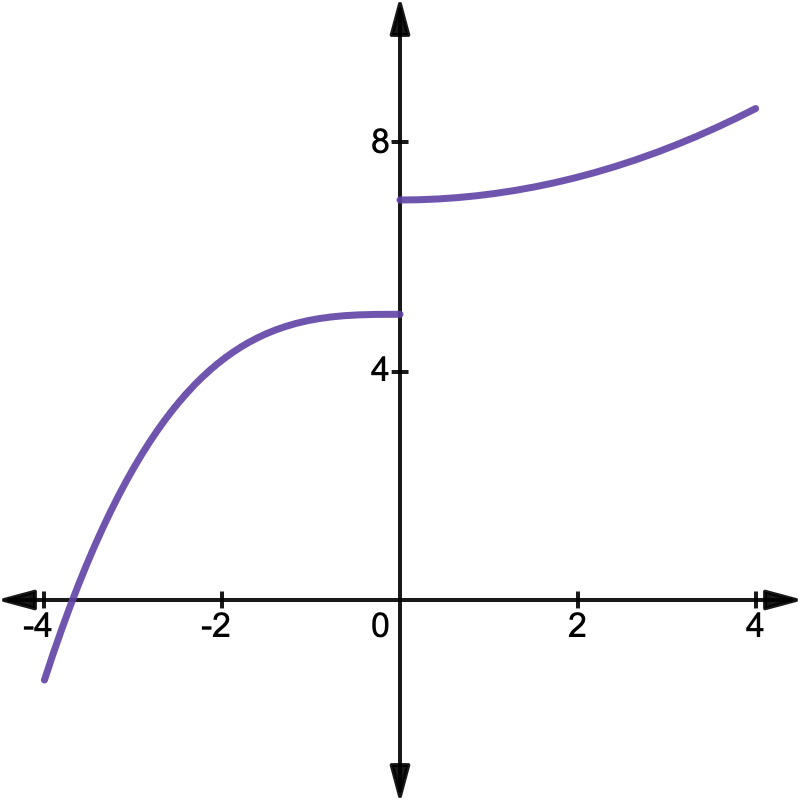
\includegraphics[scale=0.25]{input/lim1.png}	
\end{center}

\textit{Example}.  Let's calculate the limit of the following function at $x=1$.
$$f(x)\ =\ \frac{4(x-1)}{\left|x-1\right|} $$
To calculate the left-side limit plug in a value of $x$ just a tiny bit below 1, e.g. 0.99. Similarly, to calculate the right-side limit plug in a value of $x$ just a tiny bit above 1, such as 1.01. Then we can find that:
$$\lim_{x \rightarrow 1^-} f(x) = -4$$

$$\lim_{x \rightarrow 1^+} f(x) = 4$$ 
Since the left-side and right-side limit are not equal to each other, we will say that the limit of this function does not exist at 1. The graph of this function is presented below:

\begin{center}
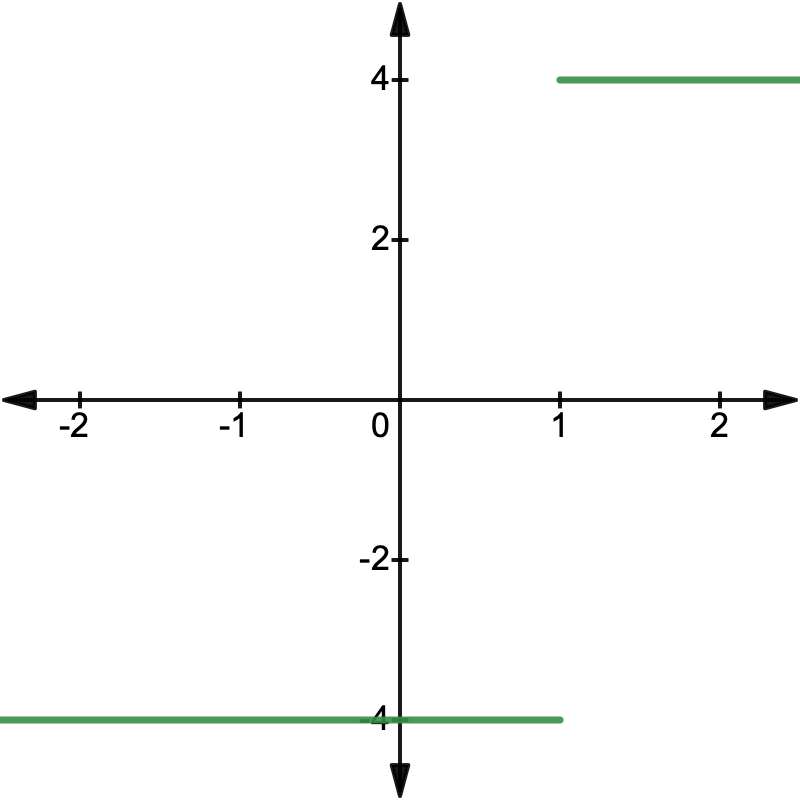
\includegraphics[scale=0.25]{input/lim2.png}	
\end{center}

%%%%%%%%%%%%%%%%%%%%%%%%%%%%%%%%%%%%%% Continuity of a Function
\section{Continuity of a Function}
A function $y=f(x)$ is said to be continuous at $a$ if the limit of $f(x)$ at $a$ exists and is equal to the value of the function at $a$ i.e.,
$$\lim _{x \rightarrow a} f(x) = f(a)$$

\textit{Example.} For the function,
$$ y = \begin{cases} 2x+1 &  \text{ if }x<1 \\
2 & \text{ if } x=1 \\
2x+1  &\text{ if }x>1 \end{cases} $$
The limit for this function exists at 1 as both the left-side limit and the right-side limit at 1 for this function is 3. But this function is not continuous because it takes value 2 when $x=1$. \\~\\

\textit{Continuity vs differentiability:} \\

$f'(x_0)$ exists if the following limit exists: 
$$  f'(x_0)= \lim_{ x \rightarrow x_0} \frac{f(x)-f(x_{0})}{x-x_0}  $$
A function $y=f(x)$ is continuous at $x_0$ if $$\lim _{x \rightarrow x_0} f(x) = f(x_0)$$
From the two definitions, we can see that continuity is a necessary condition for differentiability, but it is not a sufficient condition. In other words, if $f$ is not continuous, it implies that $f$ is not differentiable as well. But if $f$ is continuous, $f$ could either be differentiable or not. For example, the function $y = |x|$ (presented below) is continuous but not differentiable

\begin{center}
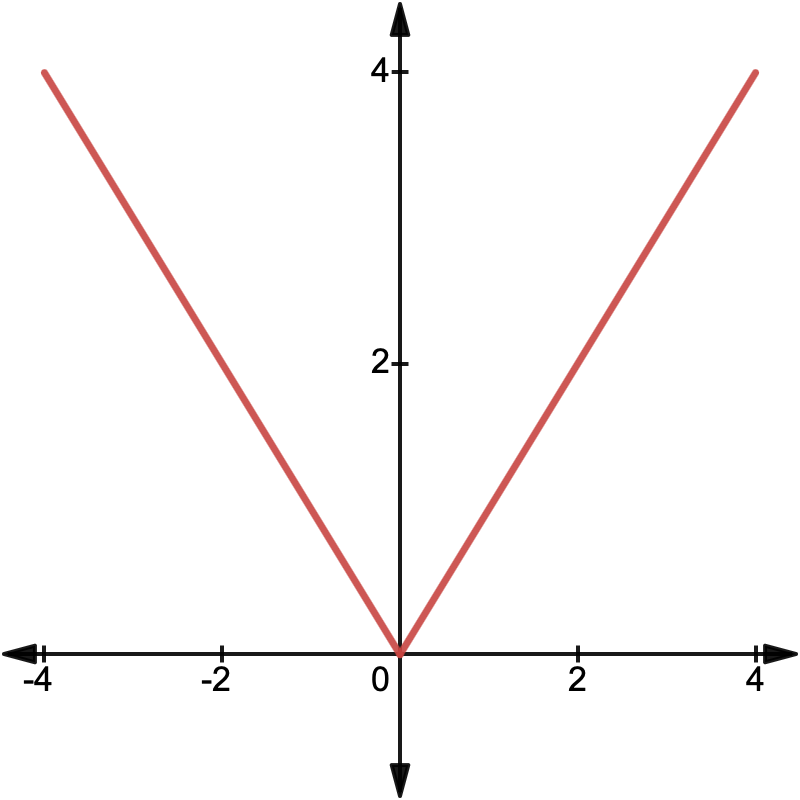
\includegraphics[scale=0.225]{input/cont_not_diff.png}
\end{center}

%%%%%%%%%%%%%%%%%%%%%%%%%%%%%%%%%%%%%% Monotonicity and inverse of a function
%\section{Monotonicity and inverse of a function}
%
%Functions that increase or decrease everywhere in their domain are called monotonic functions. Strictly increasing or decreasing functions are called strictly monotonic functions.
%\begin{itemize}
%  \item Increasing function:
%$ x_{1}>x_{2} \rightarrow f\left(x_{1}\right)\geq f\left(x_{2}\right) $ 
%\item Decreasing function:
%$ x_{1}>x_{2} \rightarrow f\left(x_{1}\right)\leq f\left(x_{2}\right) $
%\item Strictly increasing function:
%$ x_{1}>x_{2} \rightarrow f\left(x_{1}\right)>f\left(x_{2}\right) $ 
%\item Strictly decreasing function:
% $ x_{1}>x_{2} \rightarrow f\left(x_{1}\right)<f\left(x_{2}\right) $  \\
%\end{itemize}
%
%Function $y=f(x)$ has an \textit{inverse} if it is a one-to-one mapping, i.e. each value of $y$ is associated with a unique value of $x$. One-to-one mappings are unique to strictly monotonic functions. \\
%
%\textit{Definition.} For a function $y=f(x)$, the inverse function $x=f^{-1}(y)$ returns the value corresponding value of $x$ for each $y$. \\
%
%\textit{Example.} The inverse of the function $y=f(x)=2x+3$, is given by $f^{-1}(y) = (y-3)/2$ or $g(x) = (x-3)/2$. 

%%%%%%%%%%%%%%%%%%%%%%%%%%%%%%%%%%%%%% Partial Derivatives
\section{Partial Derivatives}

For a function of several variables:
$$
y=f\left(x_{1}, x_{2}, \cdots, x_{n}\right)
$$

If $x_1$ changes by $\Delta x_1$ but all other variables remain constant: 
$$
\frac{\Delta y}{\Delta x_{1}}=\frac{f\left(x_{1}+\Delta x_1, x_{2}, \cdots, x_{n}\right)-f\left(x_{1}, x_{2}, \cdots, x_{n}\right)}{\Delta x_{1}}
$$
Partial derivative of $y$ with respect to $x_i$ is defined as:
$$
\frac{\partial y}{\partial x_{i}}= f_i = \lim _{\Delta x_{i} \rightarrow 0} \frac{\Delta y}{\Delta x_{i}}
$$
Note that here, we use $\partial$ to differentiate partial derivatives from total derivatives. In particular, 
$$\left.\frac{\partial f}{\partial x_{i}} = \frac{d f}{d x_{i}} \right\vert_{\text{other variables are constant}} $$ \\

\textit{Example}. Given the production function $ Q = A K^{\alpha} L^{1-\alpha} $. \\
Marginal product of capital (MPK):
	$$\frac{\partial Q}{ \partial K} = Q_K =  \alpha A K^{\alpha-1}L^{1-\alpha}  =  \frac{\alpha Q}{K} $$

Marginal product of labor (MPL):
	$$\frac{\partial Q}{ \partial L} = Q_L = \alpha A K^{\alpha}L^{-\alpha}  =  \frac{(1-\alpha) Q}{L}$$ \\

The \textit{gradient} of a function is defined as the vector of all partial derivatives of the function:

$$ \nabla f(x_1, x_2, \cdots, x_n) = [f_1, f_2, \cdots, f_n]' $$ \\


With many functions, we can define the Jacobian matrix. Consider $n$ differentiable functions in $n$ variables that are not necessarily linear.
$$
\begin{gathered}
y_{1}=f^{1}\left(x_{1}, x_{2}, \cdots, x_{n}\right) \\
y_{2}=f^{2}\left(x_{1}, x_{2}, \cdots, x_{n}\right) \\
\cdots \\
y_{n}=f^{n}\left(x_{1}, x_{2}, \cdots, x_{n}\right)
\end{gathered}
$$ \\
The Jacobian matrix is defined
$$
J=\frac{\partial\left(y_{1}, y_{2}, \cdots, y_{n}\right)}{\partial\left(x_{1}, x_{2}, \cdots, x_{n}\right)}=\left[\begin{array}{llll}
\frac{\partial y_{1}}{\partial x_{1}} & \frac{\partial y_{1}}{\partial x_{2}} & \cdots & \frac{\partial y_{1}}{\partial x_{n}} \\
\frac{\partial y_{2}}{\partial x_{1}} & \frac{\partial y_{2}}{\partial x_{2}} & \cdots & \frac{\partial y_{2}}{\partial x_{n}} \\
\vdots & \vdots & \vdots & \vdots \\
\frac{\partial y_{n}}{\partial x_{1}} & \frac{\partial y_{n}}{\partial x_{2}} & \cdots & \frac{\partial y_{n}}{\partial x_{n}}
\end{array}\right] 
$$ \\~\\
The $n$ functions $f^{1}, f^{2}, \ldots f^{n}$ are functionally (linear or nonlinear) dependent if and only if the jacobian $|J|=0$ for all values of $x_{1}, x_{2}, \cdots, x_{n}$.

%%%%%%%%%%%%%%%%%%%%%%%%%%%%%%%%%%%%%% Differentials
\section*{Differentials}
Note that, 
$$
\Delta y \equiv\left[\frac{\Delta y}{\Delta x}\right] \Delta x
$$ 
Then for infinitesimal changes we can write,
$$
d y \equiv\left[\frac{d y}{d x}\right] d x \quad \text {or} \quad d y=f^{\prime}(x) d x
$$ 
We call $d y$ and $dx$ differentials of $y$ and $x$, respectively. We can think of $f'(x)$ as a ratio of two quantities $ dy $ and $dx$. \\

\textit{Elasticity} of function is defined as:
\[ \varepsilon = \frac{\text{Percentage change in y}}{\text{Percentage change in x}} = \frac{dy/y}{dx/x} \] 

We can calculate the elasticity by taking the derivative of $y$ with respect to $x$ as follows:
\[ \varepsilon = \frac{dy}{dx} \cdot \frac{x}{y} \]
\begin{itemize}
	\item $\varepsilon>1$, elastic
	\item $\varepsilon=1$, unit elasticity
	\item $\varepsilon<1$, inelastic \\
\end{itemize}

\textit{Example.} For the consumption function $ C = a + bY $, the elasticity is $\varepsilon = b Y/(a+bY)$. \\

For a function of $n$ variables, we can define the \textit{total differential}. For the function,  $y=f\left(x_{1}, x_{2}, \cdots, x_{n}\right)$, the total differential is given by:
\[
d f=\frac{\partial f}{\partial x_{1}} d x_{1}+\frac{\partial f}{\partial x_{2}} d x_{2}+\cdots+\frac{\partial f}{\partial x_{n}} d x_{n}=\sum_{i=1}^{n} f_{i} d x_{i}
\] \\


\textit{Example.} Consider the savings function $S=S(Y, i)$ where $S$ is savings, $Y$ is national income, and $i$ is the interest rate. Total differential is given by:
\[ 
d S=\frac{\partial S}{\partial Y} d Y+\frac{\partial S}{\partial i} d i
\] \\

The \textit{total derivative} of the $f$ with respect to $x_1$ can be obtained by dividing the total differential $df$ by $dx_1$ as follows:
\[
\frac{d f}{d x_1}=\frac{\partial f}{\partial x_{1}} +\frac{\partial f}{\partial x_{2}} \frac{d x_{2}}{d x_1}+\cdots+\frac{\partial f}{\partial x_{n}} \frac{d x_{n}}{d x_1} = f_1 +f_2\cdot \frac{d x_{2}}{d x_1}+\cdots+f_n \cdot\frac{d x_{n}}{d x_1} \]

In the case where $x_j$ does not depend on $x_1$, the term corresponding to $x_j$ will not enter the total differential as $d x_j/d x_1 = f_j= 0$. For example, if none of the other variables depend on $x_1$, the total derivative will be equal to the partial derivative. 
\[ \frac{d f}{d x_1} = \frac{\partial f}{\partial x_{1}} = f_1 \] \\

\textit{Example 1.} Suppose we have  $y = f(x_1, x_2)$ and $x_2 = g(x_1)$. In this case the total derivative of $y$ with respect to $x$ is given by:
\[ \frac{d f}{d x_1} = f_1+f_2 \cdot g'(x_1) \] \\

\textit{Example 2.} Given $y=f\left(x_{1}, x_{2}, w\right), x_{1}=g(w),$ and $x_{2}=h(w)$. The total derivative of $f$ with respect $w$ is given by:
\[ \frac{d f}{d w} = f_1 \cdot g'(w) +f_2 \cdot h'(w)  + f_3 \] \\
In this example, if instead we had $y=f(x_1, x_2)$, we could still use the definition of total derivative and just plug-in $f_3=0$ as in this case the function does not directly depend on $w$. 

%%%%%%%%%%%%%%%%%%%%%%%%%%%%%%%%%%%%%% Implicit Function Theorem
\section*{Implicit Function Theorem}

We can write an \textit{explicit} function $y=f\left(x_{1}, x_{2}, \cdots, x_{n}\right)$, as an implicit function:
\[F\left(y, x_{1}, x_{2}, \cdots, x_{n}\right)=y-f\left(x_{1}, x_{2}, \cdots, x_{n}\right)=0\] \\
\textit{Example.} For the explicit function $y = f (x_1, x_2) = x_1+3x_2-2$, we can find the implicit function $F(y, x_1, x_2) = y-x_1 -3x_2+2.$\\

However, it is not always true that for every explicit function an implicit function exists. The conditions when an implicit function exists are given by the Implicit Function Theorem stated below for the two variable case. \\

\textit{Implicit Function Theorem}

Given, $F\left(y, x \right)=0$, if the following conditions are met:
\begin{itemize}
  \item $F_y$ and $F_x$ are continuous, and
  \item at some point $x_0, y_0$ where $F(x_0,y_0) = 0$, $F_y$ is non-zero 
\end{itemize}
Then in a neighborhood around $x_0$, an implicit function exists. Moreover, this function is continuous and has continuous partial derivatives. \\

Also, when an implicit function exists, we can find its derivatives from the derivatives of the explicit function. Taking the total differential of $F\left(y, x_{1}, x_{2}, \cdots, x_{n}\right)=0$,
$$
F_{y} d y+F_{1} d x_{1}+\cdots+F_{n} d x_{n}=0 
$$

\vspace{1em}
Now suppose only $y$ and $x_{1}$ are allowed to vary, then $F_2=F_3=...=F_n=0$ and we have:
$$
F_{y} d y+F_{1} d x_{1} = 0 \quad \rightarrow \quad \frac{\partial y}{\partial x_{1}}=-\frac{F_{1}}{F_{y}} .
$$
In the simple case where the given equation is $F(y, x)=0$, the rule gives
$$
\frac{d y}{d x}=-\frac{F_{x}}{F_{y}} .
$$

\end{document}

\chapter{Exponential and Logarithmic Functions}
\documentclass{./../Latex/handout}
\begin{document}
\thispagestyle{plain}
\myheader{Exponential and Logarithmic Functions}


\textit{Reference:} Chiang, Alpha C, and Wainwright K. (2005), Fundamental Methods of Mathematical Economics: 4th edition, Chapter 10 \\

Exponential and logarithmic functions have important applications in economics. So we will discuss some basic properties and derivatives for these functions.

\subsection*{Exponential Functions}
The exponential or power function can be represented as:
$$
y=f(t)=b^{t} \quad(b>1)
$$
where $b$ denotes a fixed base of the exponent. Note that $y$ is a function of $t$, i.e. the power of $b$. A more generalized version can be written as:
$$
y=a b^{c t}
$$ \\
When the base is a special mathematical constant called Euler's number $e=2.71828...$, i.e.
$$
y=a e^{r t}
$$
it is referred to as the natural exponential function (though common to just refer to it as the exponential function as most other exponential functions don't show up as often). It is also common to write it as:
$$
y=a \exp (r t)
$$ 
\\
Where did this number $e$ come from? It can be shown that:
$$
e \equiv \lim _{n \rightarrow \infty}\left(1+\frac{1}{n}\right)^{n}
$$
Jacob Bernoulli discovered this constant in 1683 while studying a question about compound interest. \\

Suppose you invest A dollars at a 5\% interest rate that compounds yearly. After one year you will have:

\[ A \left(1+0.05\right)  \] 

After $t$ years:
\[ A \left(1+0.05\right)^{t} \]
Now rewrite the expression above as:
\[ A\left( \underbrace{\left(1+\frac{1}{1/0.05}\right)^{1/0.05}}_{\approx e} \right)^{0.05t} \approx A e^{0.05t}  \]
More generally, if $A$ is the initial principal, $r$ is the interest rate, and $t$ is the investment horizon, then the principal at $t$:
$$ A_t \approx A_0 e^{rt} $$

\subsection*{Logarithmic Functions}
Since the exponential function is a monotonic function, its inverse exists. The inverse of the exponential function is called the log or logarithmic function.\\

For the exponential function: 
\[ y=b^{t} \rightarrow log_b(y) = t  \]
where the expression on the right-hand side is referred to as the $log$ of $y$ to base $b$. For the natural exponential function:
\[y=e^{t} \rightarrow \log _{e} y =ln(y) \]

Since the natural log is employed quite often, we can write it without the base as $ln$. If you say log of $x$, without mentioning the base, it is sort of assumed that you are talking about the natural log. \\

For example, since $2^{3}=8$. So we can write $\log _{3} 8=2$. \\

Since $y=b^{t} \Longleftrightarrow t=\log _{b} y$, we can write
$$
b^{\log _{b} y}=b^{t}=y
$$

Figure 1 presents plots for $y = e^x = exp(x)$ and $y=ln(x)$. From the plots, we can see that both log and exponential functions are strictly monotonically increasing. In addition,
\begin{itemize}
	\item $y=1$, $log(y) = 0$
	\item $0<y<1$,  $\log y<0$
	\item $\log y \rightarrow \infty$ as $y \rightarrow \infty$
	\item $\log y \rightarrow-\infty$ as $y \rightarrow 0$
\end{itemize}


\pgfplotsset{%
    width=7cm,
    height=6cm
}
\begin{figure*}[t]
\begin{subfigure}[b]{0.5\textwidth}
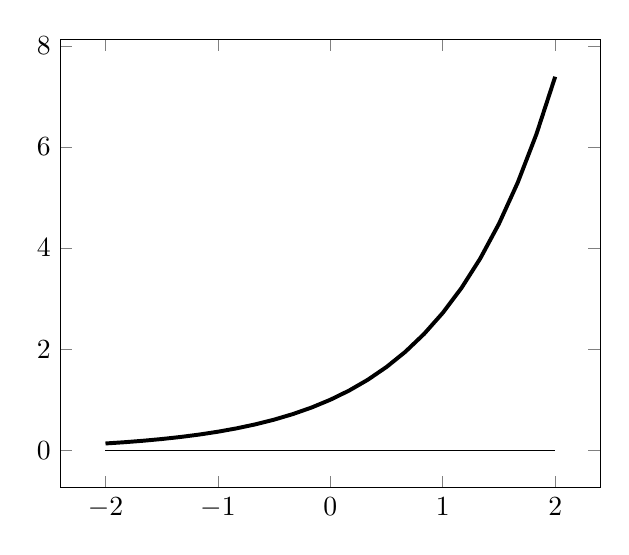
\begin{tikzpicture}
\begin{axis}[]
\addplot[color=black, line width=0.5mm, domain=-2:2] {exp(x)};
\addplot[domain=-2:2] {0};
\end{axis}
\end{tikzpicture} 
\caption{$y = e^x$}
\end{subfigure}
\begin{subfigure}[b]{0.5\textwidth}
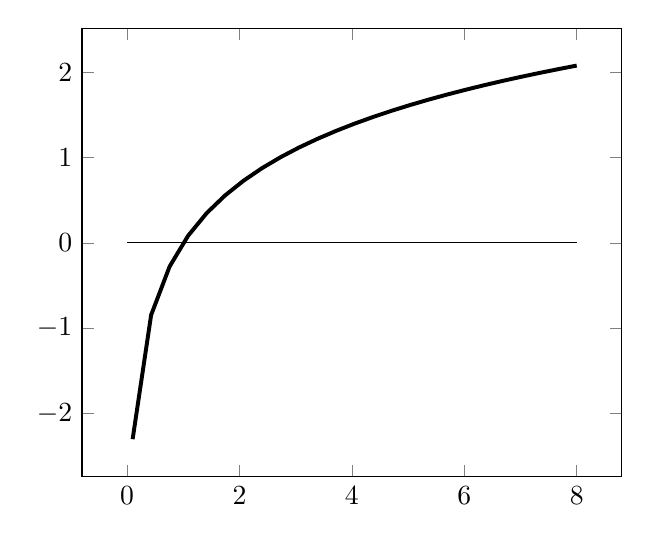
\begin{tikzpicture}
\begin{axis}[]
\addplot[color=black, line width=0.5mm, domain=0.1:8] {ln(x)};
\addplot[domain=0:8] {0};
\end{axis}
\end{tikzpicture} 
\caption{$y =ln(x)$}
\end{subfigure}
\caption{Plots for exponential and logarithmic functions}
\end{figure*}


\section*{Rules for Logarithmic Functions}
\begin{itemize}
	\item $\ln (u v)=\ln u+\ln v$ 
	\item $\ln (u / v)=\ln u-\ln v$
	\item $\ln u^{a}=a \ln u$
\end{itemize}

To see why the above rules hold, let $\ln u = s$ and $\ln v = t$. Then, $u=e^s$ and $v=e^t$. In which case,
\[ uv = e^s e^t = e^{s+t} \rightarrow \ln uv =s+t = \ln u + \ln v \]
Similarly, 
\[ u/v = e^s/e^t = e^{s-t} \rightarrow \ln (u/v) =s-t = \ln u - \ln v \]
Finally for the last rule, 
\[u^a = (e^s)^a=e^{as} \rightarrow \ln u^a = as = a\ln u \]

\section*{Derivatives of Exponential and Logarithmic Functions}
Derivative of the exponential function:
\[ y=b^{t} \quad \rightarrow \quad \frac{dy}{dt} = b^t \ln b  \]

Derivative of the generalized exponential function:
 $$y=e^{f(t)} \quad \rightarrow \quad \frac{dy}{dt} = f'(t) e^{f(t)}$$
 
Derivative of the log function:
 $$ \frac{d}{d t} \ln f(t) =\frac{f'(t)}{f(t)} $$ \\
 
\textit{Let's find the derivatives for the following functions:}
\begin{enumerate}
\item $f(t)=e^t$, $f'(t) = e^t$
\item $f(t)=\ln t$, $f'(t) = 1/t$
\item $f(t)=ae^{rt}$, $f'(t) = are^{rt}$
\item $f(t)=e^{-t}$, $f'(t) = -e^{-t}$
\item $f(t)=\ln a t$, $f'(t) = a/at = 1/t$
\item $f(t)=\ln t^{c}$, $f'(t) = ct^{c-1}/t^c = c/t$
\end{enumerate}


\end{document}

\chapter{Optimization}
\documentclass{./../Latex/handout}
\begin{document}
\thispagestyle{plain}
\myheader{Optimization}

Optimization is the process of finding the best solution to a problem, given a set of constraints and objectives. In economics, optimization plays a central role in understanding how individuals, firms, and governments make decisions to allocate scarce resources efficiently. In the context of functions, optimization involves finding a function's maximum or minimum value. 

\vspace{-1em}
%%%%%%%%%%%%% Global vs. Local Extrema
\subsection*{Global vs. Local Extrema}
\begin{itemize}
  \item Local maximum: A point where the function attains its \textit{highest} value within a neighborhood. 
 \item Local minimum: A point where the function attains its \textit{lowest} value within a neighborhood.
 \item Global (or absolute) maximum: A point where the function attains its \textit{highest} value over the entire domain.
 \item Global (or absolute) minimum: A point where the function attains its \textit{lowest} value over the entire domain.
 \end{itemize}
 
 % FIGURE: Global vs local
\begin{center}
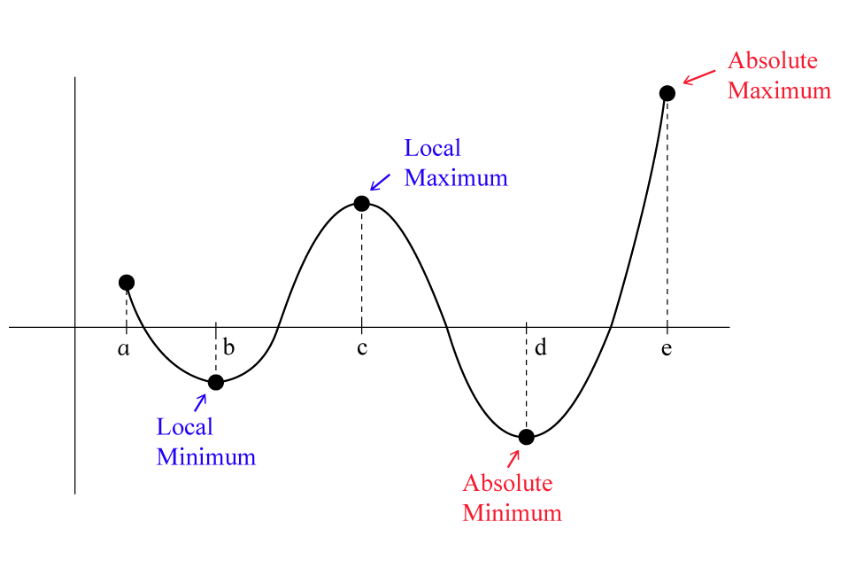
\includegraphics[scale=0.4]{./Input/global_vs_local.png}	\\
\end{center} 

Note that all global extrema are also considered local extrema. Furthermore, there can be multiple local and global extrema for a function. For example, consider the constant function $f(x) = 2$. In this case, all points in the function's domain are global maxima and global minima. There are also functions that have no extremum points, such as $f(x)=x$, which continuously increases as $x$ increases and continuously decreases as $x$ decreases, without reaching any peak or valley.

%%%%%%%%%%%%%%%%%%%%%%%%%%%%%%%%%%%%%%%%%%%%%%%%%%%%%%%%%%
% Unconstrained Optimization with One Variable
%%%%%%%%%%%%%%%%%%%%%%%%%%%%%%%%%%%%%%%%%%%%%%%%%%%%%%%%%%

\section{Unconstrained Optimization with One Variable}

We will start with the simple case of finding a maximum or a minimum of a single-variable function.  First, we will cover the first and second-order conditions for identifying the local maxima or minima of a function. We will then briefly discuss the conditions necessary for identifying global extrema.

%%%%%%%%%%%% First and Second-Order Conditions

\subsection{First and Second-Order Conditions}
 
As illustrated in the figure above, our objective is to locate the peaks or valleys of a function.  Since the derivative captures the rate of change of a function, the derivative of the function at peaks and valleys should be equal to zero. This is because the function is relatively flat in the small neighborhood of the peak or valley. 

We define a critical point as a point where the function's derivative is equal to zero. All local maxima and minima of a function, if any, must occur at critical points where the derivative of the function is equal to zero. \\

% BOX: Critical point
\fbox{\begin{minipage}{\textwidth}
The \textit{necessary} condition for $x^*$ to be a maximum or minimum point of a continuously differentiable function $f(x)$ is: \\
$$f'(x^*) = 0$$ 

Here, $x^*$ is called a critical/stationary point. 
\end{minipage}}\\

\noindent\textit{Example.} Let's find all the critical points for the function $f(x) = x^2 -24 x + 36 $. \\
We start by taking the derivative of $f(x)$: $$f'(x) = 2x-24$$
Next, we set $f'(x)$ equal to zero and solve for $x$. $2x-24=0 \rightarrow x =12$. Therefore, the critical point of $f(x)$ is $x^* = 12$.   \\

Note that it is necessary that at any maxima or minima, the derivative of the function is 0. To see this, consider a point $c$ where $f'(c)>0$, so the function is increasing at point $c$. Then the value of the function at a point just to the left of $c$ will be smaller than $f(c)$, so $c$ cannot be a local minimum. Similarly, the value of the function at a point just to the right of $c$ will be greater than $f(c)$, so $c$ cannot be a local maximum. 

While being a critical point is a necessary condition, it is not a sufficient condition for maxima or minima. This means that at any maximum or minimum point, the derivative of the function must be equal to zero. However, simply having a zero derivative at a point is not enough to conclude that the point is a maximum or a minimum. In some cases, the function may have an \textit{inflection} point or a flat spot, as shown in the following figure.

% FIGURE: Inflection point
\begin{center}
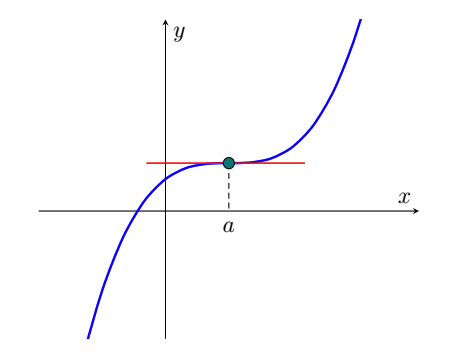
\includegraphics[scale=0.55]{./Input/inflection.png} \\
\end{center} 

Furthermore, even if we have identified a critical point that is not an inflection point, we still cannot tell whether it is a maximum or a minimum point. To determine whether the point is indeed a maximum, a minimum, or neither, we need to analyze the behavior of the function in the neighborhood of the critical point. For instance, when we are at a peak, it should be the case that the function was increasing on the left side of the critical point $x^*$ and decreasing on the right side. In other words, the derivative of the function was positive on the left side of $x^*$ and negative on the right side. This approach is called the first derivative test. \\

% BOX: First Derivative Test
\fbox{\begin{minipage}{\textwidth}
\textit{First Derivative Test} \\~\\
Suppose $f^{\prime}\left(x_{0}\right)=0$, then $x^*$ is a 
\begin{itemize}
  \item maximum if $f^{\prime}(x)$ goes from $+$ to $-$ in the immediate neighborhood of $x_{0}$ 
  \item minimum if $f^{\prime}(x)$ goes from $-$ to $+$ in the immediate neighborhood of $x_{0}$ 
  \item not an extreme point if $f^{\prime}(x)$ has the same sign in the immediate neighborhood of $x_{0}$
\end{itemize}
\end{minipage}}\\

% FIGURE: First Derivative Test
\begin{center}
\begin{tikzpicture}[scale=1.35, transform shape]
\begin{axis}[axis lines = center, ymax=3, xtick, ytick, ymin=-2, xmin=-35, xmax=65]
\addplot [domain=-30:60, samples=100, line width = 0.3mm]
{cos(5*x+2)+cos(2*x+2)};
\draw[dashed,red] (250,400) -- (450,400) node[above, yshift=-2, xshift=0] {\scriptsize $f'(x)=0$};
\draw[dashed,red] (650,120) -- (850,120)node[above, yshift=-20, xshift=-12] {\scriptsize $f'(x)=0$};
\node[right, rotate=-60, red] at (480,370) {\scriptsize $f'(x)<0$};
\node[right, rotate=60, red] at (100,255) {\scriptsize $f'(x)>0$};
\node[right, rotate=-30, red] at (480,200) {\scriptsize $f'(x)<0$};
\node[right, rotate=30, red] at (825,120) {\scriptsize $f'(x)>0$};
\end{axis}
\end{tikzpicture} \\
\end{center} 

\textit{Example.} For the function $f(x) = x^2 -24 x + 36 $, with the derivative $f'(x)=2x-24$, the critical point is $x^*=12$. Consider a point just below $12$, say $x=11.99$. The derivative at this point is $f'(11.99)=2(11.99)-24=-0.02<0$. Now consider a point just above $12$, say $x=12.01$. The derivative at this point is $f'(12.01)=2(12.01)-24=0.02>0$. So the function is decreasing as $x$ approaches $x^*$ and then starts increasing beyond $x^*$. So we can conclude that the critical point $x^*=12$ corresponds to a valley or a local minimum. \\

Instead of checking whether the derivative goes from positive to negative, we can also just look at the sign of the second derivative at the critical point, which is often easier. This is called the second derivative test. \\

\fbox{\begin{minipage}{\textwidth}
\textit{Second Derivative Test} \\~\\
Suppose $f^{\prime}\left(x_{0}\right)=0$, then $x^*$ is a 
\begin{enumerate}
  \item a maximum if $f''(x^*)<0$
  \item a minimum if $f''(x^*)>0$ 
\end{enumerate}
\end{minipage}} \\

The second derivative of a function is the derivative of the first derivative, and, hence it measures the rate of change of the first derivative. Consider a critical point $x^*$. When $f''(x^*)<0$, it means that $f'(x)$ is decreasing in the neighborhood of $x^*$. Since $f'(x^*)=0$ and $f'(x)$ is decreasing in the neighborhood of $x^*$, it must be that the sign of $f'(x)$ changes from positive to negative at $x^*$, indicating a local maximum. Similarly, when $f''(x^*)>0$, it means that $f'(x)$ is increasing at $x^*$, and it must be that $f'(x)$ changes from negative to positive at $x^*$, indicating a local minimum. \\

\textit{Example.} For the function $f(x) = x^2 -24 x + 36 $, with the derivative $f'(x)=2x-24$, the critical point is $x^*=12$. The second derivative is given by, $ f''(x) = 2 $, which is positive at all points, including at $x=12$. So from the second derivative test, we can conclude that $12$ is a local minimum. \\

Finally, note that if $f'(x^*)=0$ and $f''(x^*)>0$ or $f''(x^*)<0$, then we have a sufficient condition for determining whether $x^*$ is a maximum or minimum point. However, this condition is not necessary, as there are cases where $f''(x^*)=0$, and yet $x^*$ is a maximum or minimum point. An example of such a case is the function $f(x)=x^4$, with $f'(x)=4x^3$ and $f''(x)=12x^2$. The critical point for this function is at $0$ and $f''(0)=0$, yet $0$ is the minimum point. The graph of this function is presented below. 

% FIGURE: y=x^4
\begin{center}
	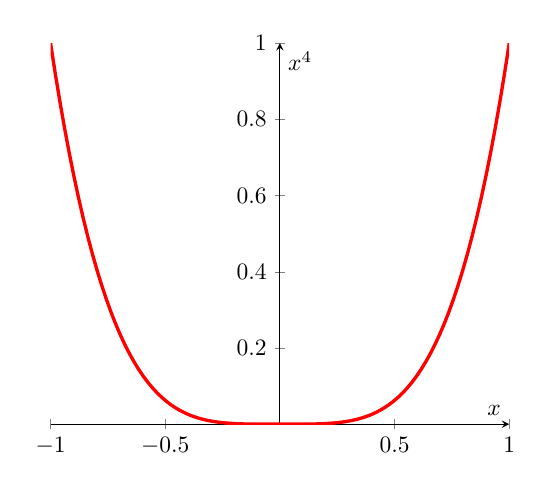
\begin{tikzpicture}[scale=0.85, transform shape]
\begin{axis}[axis lines = center, xlabel = \(x\), ylabel = \(x^4\)]
\addplot [domain=-1:1, samples=100, color=red, line width = 0.5mm]
{x^4};
\end{axis}
\end{tikzpicture} \\
\end{center}

Alternatively, we can say that $f'(x^*)=0$ and $f''(x^*) \geq 0$ or $f''(x^*)\leq 0$ is the necessary condition for determining whether $x^*$ is a maximum or minimum point.  

The following table summarizes the first and second-order conditions for local maximum and minimum. \\

\begin{tabularx}{\textwidth}{lXX}
\hline Condition & Maximum & Minimum \\
\hline \\ 
First-order necessary & $f^{\prime}(x)=0$ & $f^{\prime}(x)=0$ \\~\\
Second-order necessary ${ }^{\dagger}$ & $f^{\prime \prime}(x) \leq 0$ & $f^{\prime \prime}(x) \geq 0$ \\~\\
Second-order sufficient ${ }^{\dagger}$ & $f^{\prime \prime}(x)<0$ & $f^{\prime \prime}(x)>0$ \\~\\
\hline
\end{tabularx} \\
${ }^{\dagger}$ Applicable only after the first-order necessary condition has been satisfied.
\vspace{0.25em}

%%%%%%%%%%%% Conditions for Global Extrema

\subsection{Conditions for Global Extrema}
The conditions for global extrema are similar to those for local extrema, but now we need to look at the sign of $f''(x)$ over the entire domain of the function and not just locally at $x^*$. In particular, if $f''(x)<0$ for all $x$ in the domain of $f$, then any critical point of $f$ is a unique global maximum. This is because $f'(x)$ is decreasing over the entire domain of $x$, and can only be 0 at a unique critical point where it goes from positive to negative, implying that it is the unique global maximum. 

At this point, it is useful to define concave and convex functions. \\

\fbox{\begin{minipage}{\textwidth}
\begin{itemize}
  \item A function $f(x)$ is said to be \textit{concave} if  $ f''(x) \leq 0$ for all $x$.
  \item A function $f(x)$ is said to be \textit{convex} if  $ f''(x) \geq 0$ for all $x$.
\item A function $f(x)$ is said to be \textit{strictly concave} if  $ f''(x) < 0$ for all $x$.
  \item A function $f(x)$ is said to be \textit{strictly convex} if  $ f''(x) > 0$ for all $x$.
\end{itemize}
\end{minipage}} \\

So now, we can write the conditions for global extrema in terms of concave and convex functions. \\

\fbox{\begin{minipage}{\textwidth}
\begin{itemize}
  \item If a function is (strictly) concave, any critical point will give us a (unique) global maximum.
  \item If a function is (strictly) convex, any critical point will give us a (unique) global minimum.
\end{itemize}
\end{minipage}} \\

Since concave and convex functions allow flat regions, it is possible for there to be multiple extrema. This was the case in our example with $f(x)=2$, which is both a concave and a convex function as $f''(x)=0$. 

%%%%%%%%%%%%%%%%%%%%%%%%%%%%%%%%%%%%%%%%%%%%%%%%%%%%%%%%%%
% Unconstrained Optimization with Multiple Variables
%%%%%%%%%%%%%%%%%%%%%%%%%%%%%%%%%%%%%%%%%%%%%%%%%%%%%%%%%%

\section{Unconstrained Optimization with Multiple Variables}

In economics, we often encounter situations where we need to maximize a function that involves more than one variable. For example, we may want to determine the optimal quantity of two or more inputs, such as labor and capital, that a firm should use to produce a given level of output. 

To solve for the optimal values of multiple input variables, we need to take the partial derivative of the output function with respect to each input variable and set them equal to zero. This is the first-order condition (FOC) for multivariate functions. 

 For a function of two variables $f(x,y)$, the FOC is given by:
$$ f_x = \frac{\partial f}{\partial x} = 0 , \quad \quad f_y = \frac{\partial f}{\partial y} = 0 $$
Here, $f_x$ and $f_y$ are the partial derivatives of $f$ with respect to $x$ and $y$, respectively. In particular, $f_x$ captures, how $f$ changes as $x$ changes while holding $y$ constant. So when calculating the partial derivative with respect to one variable, we treat the other variable as a constant. \\

\textit{Example.} Let's find all the critical points for the function $$f(x,y) = x + y^2- x^2y$$ 
Note that, $f_x=1-2xy$ and $f_y = 2y-x^2$. 
Setting $f_x=0$, we get $xy=0.5$ and setting $f_y=0$, we get $y=0.5x^2$. 
Plugging $y=0.5x^2$ in  $xy=0.5$, we get at $x=1$ and $y=0.5$. So the critical point for this function is $(1,0.5)$. \\

\textit{Example.}  Consider the profit function $\pi(K,L) = Q(K,L) - rK - wL$, where $Q(K,L)$ is the production function that specifies the maximum quantity of output that can be produced using $K$ units of capital and $L$ units of labor. Here, $r$ and $w$ are the prices of capital and labor, respectively. 

The partial derivative of $\pi$ with respect to $L$ is given by:
 $$ \pi_L = \frac{\partial \pi}{\partial L}  = Q_L-w = 0   $$
Here, $Q_L$ is the partial derivative of the production function with respect to labor, which measures the marginal product of labor (MPL) or the increase in output resulting from an additional unit of labor. Similarly, $Q_K$ is the partial derivative of the production function with respect to capital, which measures the marginal product of capital (MPK). 

The partial derivative of $\pi$ with respect to $K$ is:
$$ \pi_K = \frac{\partial \pi}{\partial K}  = Q_K-r = 0   $$
At the critical point where both FOCs are satisfied, the firm will choose inputs so that the price of each input is equal to its marginal product. (Note that $Q_K$ and $Q_L$ are functions of $K$ and $L$.) \\

For multivariate functions, the second-order conditions involve calculating all the (own and cross) second partial derivatives of the function. We will skip details on these conditions here. However, it is important to note that the concept of concavity and convexity can be extended to multivariate functions. In particular, we can define a concave (convex) function as a function whose graph lies below (above) any line segment connecting any two points on the graph. (See the slides for Lecture 12 for more details.) Moreover, as before, any critical point of a multivariate (strictly) concave/convex function represents a (unique) global maximum/minimum. 

%%%%%%%%%%%%%%%%%%%%%%%%%%%%%%%%%%%%%%%%%%%%%%%%%%%%%%%%%%
% Constrained Optimization 
%%%%%%%%%%%%%%%%%%%%%%%%%%%%%%%%%%%%%%%%%%%%%%%%%%%%%%%%%%

\section{Constrained Optimization}
Lots of problems in economics involve optimizing a function subject to one or more constraints. For example, a firm may want to maximize its profits subject to production constraints, or a consumer may want to maximize their utility subject to a budget constraint. To solve such problems, we use the method of Lagrange multipliers. 

Suppose we want to maximize (or minimize) a function $f(x,y)$ subject to a constraint $g(x,y) = c$, where $c$ is a constant. The method of Lagrange multipliers involves constructing a new function, known as the Lagrangian, that combines the objective function and the constraint function as follows:
$$
L(x,y,\lambda)=f(x, y)+\lambda[c-g(x, y)]
$$

Here, $\lambda$ is the Lagrange multiplier. To find the optimal values of $x$ and $y$, we need to take partial derivatives of the Lagrangian with respect to each variable and the Lagrange multiplier and set them equal to zero. This gives us the first-order conditions:
\begin{align*}
L_x(x,y,\lambda) = \frac{\partial L}{\partial x} &= f_x(x, y)- \lambda \cdot g_x(x, y) = 0 \\
L_y(x,y,\lambda) = \frac{\partial L}{\partial y} &= f_x(x, y)- \lambda \cdot g_x(x, y) = 0 \\
L_{\lambda}(x,y,\lambda) = \frac{\partial L}{\partial \lambda} &= c-g(x, y) = 0 
\end{align*}
Here, $f_k$ and $g_k$ represent the partial derivative with respect to $x_k$ of the objective function and the constraint, respectively. 

Intuitively, the Lagrange multiplier method works because it allows us to take into account the constraint when optimizing the function. By introducing the Lagrange multiplier, we are effectively adding a penalty term to the objective function that accounts for the constraint. The Lagrange multiplier $\lambda$ has an economic interpretation as the shadow price of the constraint. It measures the change in the objective function resulting from a small change in the constraint function. Thus, the Lagrange multiplier provides us with information about the value of relaxing or tightening the constraint.\\


\textit{Example}. We want to maximize utility given by  $U(x,y) = x y$ subject to the budget constraint $4 x + y = 12$. 

We start by setting up the Lagrangian:
$$ L(x, y, \lambda) = x y + \lambda(12-4x-y) $$
First-order conditions:
\begin{align}
\frac{\partial L}{\partial x} &= y- 4 \lambda = 0  \\ 
\frac{\partial L}{\partial y} &= x- \lambda  = 0 \\ 
\frac{\partial L}{\partial \lambda} &= 12-4x-y = 0 
\end{align}
From equations (1) and (2), we have $y=4 \lambda$ and $x=\lambda$, which implies that $y=4x$. Plugging this in equation (3):
$$ 12-4x-4x = 0 \rightarrow x^* = 1.5, y^*=6, \lambda^* = 1.5 $$

Interpretation of $\lambda^*$: If income increases by a dollar, utility increases by $1.5$.\\

The method of Lagrange multipliers can be extended to problems with more than two variables and constraints. For example, consider the problem of maximizing a function $f(x,y,z)$ subject to two constraints $g(x,y,z) = c$ and $h(x,y,z) = m$, where $c$ and $m$ are constants. To solve this problem, we will need to introduce two Lagrange multipliers and then construct the Lagrangian function as follows:
$$L(x,y,z,\lambda,\mu) = f(x,y,z) + \lambda [c-g(x,y,z)] + \mu [m-h(x,y,z)]$$
To find the optimal values of $x$, $y$, and $z$ that maximize $f(x,y,z)$ subject to the two constraints, we can take the partial derivatives of the Lagrangian with respect to $x$, $y$, $z$, $\lambda$, and $\mu$, and set them equal to zero. 

\subsection*{Global Extrema with Constraints}

The Lagrange multiplier method transforms the constrained optimization problem of maximizing $f(x,y)$ subject to $g(x,y)$ into an unconstrained optimization problem of maximizing $ L(x, y, \lambda)$. We know that in the case of unconstrained optimization, any critical point of a concave function represents a global maximum. In the case of constrained optimization, if both $f(x,y)$ and $g(x,y)$ are concave, then $L(x,y,\lambda)$ will also be concave, and any critical point of $L(x,y,\lambda)$ will represent the global maximum of $f(x,y)$ subject to $g(x,y)$. However, requiring functions to be concave is a strong condition. We can instead use the weaker condition that $f(x,y)$ is quasiconcave, and the constraint set, $C=\{(x,y):g(x,y)=c\}$, is a convex set to ensure that we are identifying the global maximum. (See the slides for Lecture 12 for definitions.) \\

\fbox{\begin{minipage}{\textwidth}
The stationary point $(x_1^*, x_2^*, ..., x_n^*)$ of the Lagrangian corresponding to the problem of optimizing $f(x_1,x_2,..,x_n)$ subject to a constraint $g(x_1, x_2,...,x_n)=c$ is a global maximum if:
\begin{enumerate}
  \item $f(x_1,x_2,...,x_n)$ is quasiconcave
  \item The constraint set is convex\\
\end{enumerate}
\end{minipage}} \\


\section{Envelope Theorem}

In economics, we are often interested in understanding how the value of a function changes in response to certain \textit{parameters}. For example, we may be interested in how a consumer's utility changes in response to changes in prices, or how a firm's profits change in response to changes in wages. When analyzing how a function's value changes in response to changes in parameters, we need to consider both the direct impact of changing the parameters on the function's value, as well as the indirect impact of changing the parameters on the optimal inputs, which in turn affects the function's value. The Envelope Theorem tells us that we do not need to worry about the indirect effect of changing parameters on the optimal inputs --- we can simply focus on the direct effect. \\

\fbox{\begin{minipage}{\textwidth}
\textit{Envelope Theorem: Unconstrained Maximization} \\
Consider the following maximization problem: 
$$
\max_{x} \quad  f(x, \alpha)  
$$
Here, $\alpha$ is a parameter. Since the optimal input may depend on $\alpha$, let's denote it by $x^*(\alpha)$. Now let's define the \textit{maximum value function}:
$$ V(\alpha) = f(x^*(\alpha), \alpha) $$
The envelope theorem states that,
$$ V_{\alpha}= \frac{\partial V}{\partial \alpha} = f_{\alpha}^* $$
where $f_{\alpha}^*$ is the partial derivative of $f$ with respect to $x$ at $x^*$
\end{minipage}} \\

It is actually straightforward to see why this is the case. Note, that when we differentiate $V$ with respect to $\alpha$,
$$ V_{\alpha} = f_x^* \cdot \frac{\partial x^*}{\partial \alpha} + f_{\alpha}^* $$
Here, $f_x^*$ is the partial derivative of $f$ with respect to $x$ at $x^*$. By first order conditions for optimization, $f_x^*=0$, and hence $ V_{\alpha}=f_{\alpha}^* $. \\

\textit{Example.} Say we want to choose labor input $L$ to maximize profit $$\max_L \quad\pi(L, w) = \ln L-wL$$ 
Here, $w$ is the wage rate. Writing the first-order condition:
$$ \pi_L = \frac{1}{L}-w = 0 \rightarrow L^* = \frac{1}{w} $$
Since $L^*$ depends on $w$, we can write it as $L^*(w)$.

Now, we are interested in how optimal profit changes with respect to changes in wages. To answer this question, we first write down the maximum value function, which here depends on $w$. 
$$ V(w) = \pi(L^*(w), w) =  \ln L^*(w)-wL^*(w) $$
Now to see how $V(w)$ varies with $w$ we need the derivative of $V$ with respect to $w$. The envelope theorem says that this derivative is given by
$$ V'(w) =  \pi_w(L^*(w), w) =-L^*(w) = -\frac{1}{w}$$
We can also verify this by plugging in $L^*(w)=1/w$ in the expression for $V(w)$ and then differentiating with respect to $w$.
$$ V(w) =   \ln L^*(w)-wL^*(w) = \ln(1/w)-1 = \ln 1-\ln w-1 \rightarrow V'(w)=-\frac{1}{w}$$ 

The envelope theorem for constrained optimization problems is stated below. \\

\fbox{\begin{minipage}{\textwidth}
\textit{Envelope Theorem: Constrained Maximization} \\
Consider the following constrained optimization problem $$ \max_{x,y} \quad  f(x, y ; \alpha) \quad \text{s.t.} \quad G(x, y ; \alpha)=0$$ 
Lagrangian function:
$$
L(x,y,\lambda; \alpha) =f(x, y ; \alpha)+\lambda G(x, y ; \alpha)
$$
As before, define the value function $V(\alpha)=f(x^*, y^* ; \alpha)$. Then the envelope theorem states,
$$
\frac{\partial V}{\partial \alpha}=\frac{\partial L(x^*, y^*, \lambda^*; \alpha)}{\partial \alpha} $$
\end{minipage}} \\

The above theorem directly implies interpretation of the lagrange multiplier. Say max $f(x, y)$ subject to $g(x, y)=c$ 
Can think of the constraint as:
$$ G(x,y,c)= c-g(x,y) $$
So here $c$ is the parameter $\alpha$. Now what happens due to change in $c$ to the value function is given by 
$$
\frac{\partial V}{\partial \alpha}=\frac{\partial L(x^*, y^*, \lambda^*; \alpha)}{\partial \alpha} = \lambda^*$$ \\

\textit{Example}. We want to maximize the utility function $U(x_1,x_2)=x_1 x_2$ subject to the budget constraint $p_1 x_1 + p_2 x_2 = m$, where $m$ is the total income. We are interested in how the total utility changes due to a change in price of good 1. 

Setting up the Lagrangian: 
$$
L(x_1,x_2,\lambda) =x_1 x_2 + \lambda(m-p_1x_1-p_2x_2)
$$
First-order conditions:
\begin{align}
	L_{1} &= x_2-\lambda p_1=0 \\
	L_{2} &= x_1-\lambda p_2=0 \\
	L_{\lambda} &= m-p_1x_1-p_2x_2 = 0
\end{align}
Equations (4) and (5) imply that $x_2/x_1 = p_1/p_2$. Plugging $x_2 = p_1x_1/p_2$ in equation (6):
$$m-p_1x_1-p_2x_2 = m-p_1x_1-p_1x_1 \rightarrow x_1^*=\frac{m}{2p_1},x_2^*=\frac{m}{2p_2}, \lambda^* = \frac{m}{2p_1 p_2}  $$
Denote $L^*=L(x_1^*,x_2^*,\lambda^*)$. Then according to the envelope theorem how optimal utility changes with respect to $p_1$ is given by $$ \frac{\partial L^*}{\partial p_1} = -\lambda^* x_1^* = - \frac{m^2}{4p_1^2 p_2}$$

We can verify that this is true as:
$$ V(p_1,p_2,m) = x_1^* x_2^* = \frac{m^2}{4p_1 p_2} \rightarrow \frac{\partial V}{\partial p_1} = - \frac{m^2}{4p_1^2 p_2}$$

\end{document}

\chapter{Optimization Examples}
\documentclass{./../Latex/handout}
\begin{document}
\thispagestyle{plain}
\myheader{Optimization Examples}

% Example 1
\section*{Example 1: Utility Maximization}
Consider the following utility maximization problem:$$ \max_{\{x_1,x_2\}} \quad x_1^{\alpha} x_2^{\beta} \quad s.t. \quad p_1 x_1 + p_2 x_2 = m $$
 
 Here, $p_1$ and $p_2$ are the prices of goods 1 and 2, and $m$ is the total income available to spend on the two goods. 
 To find the critical points, we start by setting up the Lagrange function: 
  $$ \mathcal{L}(x_1,x_2,\lambda) =  x_1^{\alpha} x_2^{\beta} + \lambda(m-p_1 x_1-p_2 x_2)$$
  
The first-order conditions are given by:
\begin{align}
	\frac{\partial \mathcal{L}}{\partial x_1} &= \alpha x_1^{\alpha-1}x_2^{\beta}-\lambda p_1 = 0 \\ 
	 \frac{\partial \mathcal{L}}{\partial x_1} &= \beta x_1^{\alpha}x_2^{\beta-1}-\lambda p_2 = 0 \\
	  \frac{\partial \mathcal{L}}{\partial \lambda} &= m-p_1 x_1-p_2 x_2 = 0 
\end{align}

From equations (1) and (2), we have $\alpha x_1^{\alpha-1}x_2^{\beta}=\lambda p_1 $ and  $\beta x_1^{\alpha}x_2^{\beta-1}=\lambda p_2$, dividing the first expression by the second, we get:
$$ \frac{\alpha x_1^{\alpha-1}x_2^{\beta}}{\beta x_1^{\alpha}x_2^{\beta-1}} = \frac{\lambda p_1}{\lambda p_2}$$

Simplifying this expression further:
$$ \frac{\alpha x_2^{\beta}x_2^{1-\beta}}{\beta x_1^{\alpha}x_1^{1-\alpha}} = \frac{ p_1}{ p_2} \rightarrow \frac{\alpha x_2}{\beta x_1} = \frac{p_1}{p_2} $$

Then we can write that, 
$$ x_2 = \frac{\beta}{\alpha}\cdot\frac{p_1}{p_2} \cdot x_1$$

Plugging the above expression for $x_2$  in equation (3):
$$ m-p_1 x_1-p_2 x_2 = m-p_1 x_1- \frac{\beta}{\alpha}\cdot p_1 x_1 = m-p_1 x_1\left(1+ \frac{\beta}{\alpha}\right) =0  $$
So we can find, $$x^*_1 = \frac{\alpha}{\alpha+\beta}\frac{m}{p_1}$$

Plugging back $x_1$ in the expression for $x_2$, we can find:
$$x^*_2 = \frac{\beta}{\alpha+\beta}\frac{m}{p_2}$$ 

% Example 2
\section*{Example 2: Cost Minimization}
Consider the following cost minimization problem where $p$ is the price of capital, and $w$ is the price of labor. Quantity is constrained at $\bar{Q}$. 
$$ \max_{\{K,L\}} \quad p K + w L \quad s.t. \quad Q(K,L) = \bar{Q} $$

Lagrange function: 
  $$ \mathcal{L}(x_1,x_2,\lambda) =  p K + w L + \lambda(\bar{Q}-Q(K,L))$$
First-order conditions:
\begin{align*}
	\frac{\partial \mathcal{L}}{\partial K} &= p-\lambda Q_K(K,L)=0 \\ 
	 \frac{\partial \mathcal{L}}{\partial L} &= w-\lambda Q_L(K,L) = 0 \\
	  \frac{\partial \mathcal{L}}{\partial \lambda} &= \bar{Q}-Q(K,L)
\end{align*}
Note that here $Q_K = \dfrac{\partial Q}{\partial K}$ and $Q_L = \dfrac{\partial Q}{\partial L}$. \\

So optimal $K$ and $L$ satisfy:
$$ (1). \quad \frac{Q_K(K^*,L^*)}{Q_L(K^*,L^*)} = \frac{p}{w},  \quad \quad (2). \quad Q(K^*,L^*) = \bar{Q}$$ 

% Example 3
\section*{Example 3: Inter-Temporal Utility Maximization}
You are given the following inter-temporal utility function:
\begin{align}
	U = U(c_1, c_2) =  \ln c_1 + \beta \ln c_2
\end{align}
where $c_1$ and $c_2$ is consumption in period 1 and 2, respectively. $0<\beta<1$ is the rate at which you discount the future and it measures your impatient. You earn income $y_1>0$ in period 1 and income $y_2>0$ in period 2. Any of the income you save $s$ in period 1 earns interest $r>0$. So, $$ c_1 + s = y_1, \quad \quad c_2 = y_2 + (1+r) s $$
Combining these constraints:
$$ c_1 + \frac{1}{1+r} c_2 = y_1 + \frac{1}{1+r} y_2 $$
Let the present-discounted income be denoted by $m$, such that:
$$ m = y_1 + \frac{1}{1+r} y_2 $$

\vspace{1em}
You want to choose $c_1$ and $c_2$ to maximize utility $U(c_1, c_2)$ in equation (4) subject to the constraint:
 \begin{align} c_1 + \frac{1}{1+r} c_2 = m \end{align}
 
 Lagrangian function:
$$ L(c_1, c_2, \lambda) = \ln c_1 + \beta \ln c_2 + \lambda\left(m- c_1 - \frac{1}{1+r} c_2 \right) $$

First order conditions:
\begin{align}
		\frac{\partial L}{\partial c_1}&=\frac{1}{c^*_1}-\lambda^*=0 \\
		\frac{\partial L}{\partial c_2}&=\frac{\beta}{c^*_2}-\frac{\lambda^*}{1+r}=0 \\
		\frac{\partial L}{\partial \lambda}&=m- c^*_1 - \frac{1}{1+r} c^*_2=0
	\end{align}
	
Note that from (6), $\lambda^*=1/c_1^*$, plugging this in (7), we get:
$$ c_2^* = \beta(1+r)c_1^*  $$
Plugging this expression for $ c_2^*$ in (8):
$$ c_1^* + \frac{1}{1+r}\beta(1+r)c_1^* = m \rightarrow c_1^* =\frac{m}{1+\beta}  $$
In which case,
$$ c_2^* = \beta(1+r)c_1^* = \frac{\beta m(1+r)}{1+\beta}    $$
Finally, since $\lambda^*=1/c_1^*$,
$$\lambda^*=\frac{1}{c_1^*} = \frac{1+\beta}{m} $$	\\

Now suppose we are interested in knowing how utility changes due to changes in total income. By the envelope theorem:
$$ \frac{\partial U^*}{\partial m}=\frac{\partial L^*}{\partial m} = \lambda^* = \frac{1+\beta}{m} $$ \\
Similarly, how utility changes due to a change in interest rate would be given by:
$$ \frac{\partial U^*}{\partial r}=\frac{\partial L^*}{\partial r} = \lambda^*\cdot \frac{1}{(1+r)^2}\cdot c_2^* = \frac{\beta}{1+r} $$ \\

\end{document}

\end{document}
